
\section{Magnitude Estimation Relevance Judgments}
\label{sec-rq1}

Having obtained magnitude estimation scores for 4,269 topic-document
pairs, we analyze the user-perceived relevance to answer the first
research question RQ\ref{item:rq1}, whether the magnitude estimation
technique is suitable for gathering document level relevance
judgments, and whether the resulting relevance scales are reasonable
with respect to our current knowledge of relevance judgments.

\subsection{Consistency of Magnitude Estimation and Ordinal Relevance}
\label{sec:cons-magn-estim}

\begin{figure}[t]
  \centering
  \includegraphics[width=.7\linewidth,page=19]{figs/check_gross_ranks_med.pdf}
  \vspace{-0.5cm}
  \caption{ME score distribution by Sormunen and TREC levels.}
  \label{fig:ME-distribution}
\end{figure}


\begin{figure}[tp]
  \centering
  %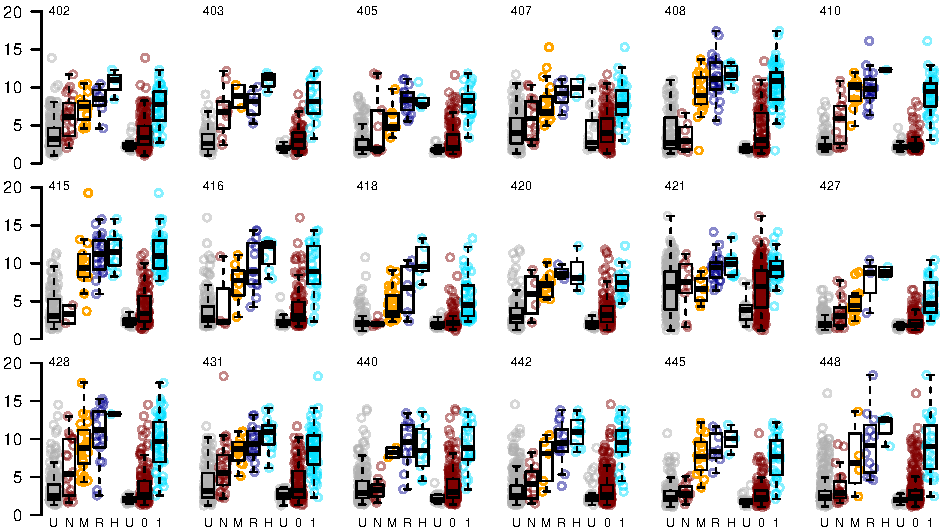
\includegraphics[angle=90,height=.9\textheight,page=1]{figs/check_gross_ranks_med_all.pdf}
  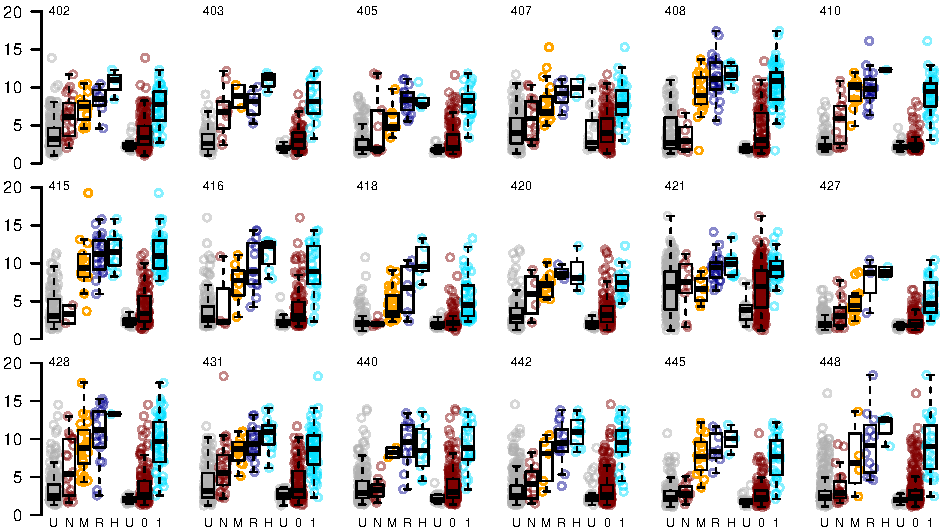
\includegraphics[width=\linewidth,page=1]{figs/check_gross_ranks_med_all.pdf} %
  \caption{ME score distribution by Sormunen (U, N, M, R, H) and TREC (U, 0, 1) levels:
    breakdown for individual topics.
  \label{fig:ME-distribution-breakdown}
   }
\end{figure}

The distribution of the median normalized magnitude estimation scores for
each document are shown in Figure~\ref{fig:ME-distribution}, aggregated
across all 18 topics, and split by Sormunen ordinal relevance levels
(left side of figure, levels are 
\nn, \mm, \rr, \hh, and {\tt U}, the group of documents that were not judged
by Sormunen), and by TREC binary levels (right side of figure, levels
are $0$, $1$, and {\tt U}, the documents that were not judged by TREC, as not all participating runs were
included in the judging pool).
This boxplot (and subsequent boxplots) show the median as a solid black
line; boxes show the 25th to 75th percentile; and whiskers show the
range, up to 1.5 times the inter-quartile range.
There is a clear distinction between each of the four adjacent
Sormunen levels, (two-tailed t-test, $p<0.002$), 
with the magnitude estimation scores on average following the
ordinal scale rank ordering.
The differences between the two TREC levels are also significant
($p<0.001$), with the magnitude estimation scores on average again being
aligned with the binary levels.
This is strong evidence for the overall validity of the 
magnitude estimation approach.


Figure~\ref{fig:ME-distribution-breakdown} shows the magnitude
estimation score distributions for
each of the 18 individual topics. 
Although there is some variability across topics, overall the figure
confirms that the magnitude estimation scores are usually aligned with
ordinal categories even when considering individual topics: the
medians of the median magnitude estimation scores (the solid black
lines) generally follow the ordinal categories, for all categories and
for all topics (there are some exceptions for some of the Sormunen
adjacent categories in topics 403, 405, 410, 420, 421, and 440; there
are no exceptions for non-adjacent categories, nor for TREC
categories). 
Since for each topic there could potentially be 3 exceptions for
adjacent categories, and 6 exceptions in general, plus one exception
for the two TREC categories, the 6 exceptions found are out of
$3 * 18 + 18 = 72$ possible cases when considering only adjacent
categories, or out of $6 * 18 + 18 = 126$ cases when considering also
non-adjacent categories. 
Such a limited fraction of exceptions (in the $5\%$-$8\%$ range) is
further strong evidence for the validity of our
approach, even at the single topic level.

Regarding the set of documents that were not judged by Sormunen
(left-most boxes in Figure~\ref{fig:ME-distribution} and sub-plots in
Figure~\ref{fig:ME-distribution-breakdown}), based on the magnitude
estimation scores it can be inferred that the bulk of this class are
likely to be non-relevant; however there are also instances that occur
across the central parts of the marginal to highly relevant score
distributions. There were also a handful of documents unjudged by 
TREC that seemed to be rated highly by our judges.
It can also be observed that while the overall distributions of
magnitude estimation scores are strongly consistent with the ordinal
and binary categories, there are also documents in each class 
where the ME scores 
fall into the central region of a different class.
We therefore next investigate judge agreement.


\subsection{Judge Agreement}
\label{sec:judge-agreement}

\begin{figure}[tp]
  \centering
  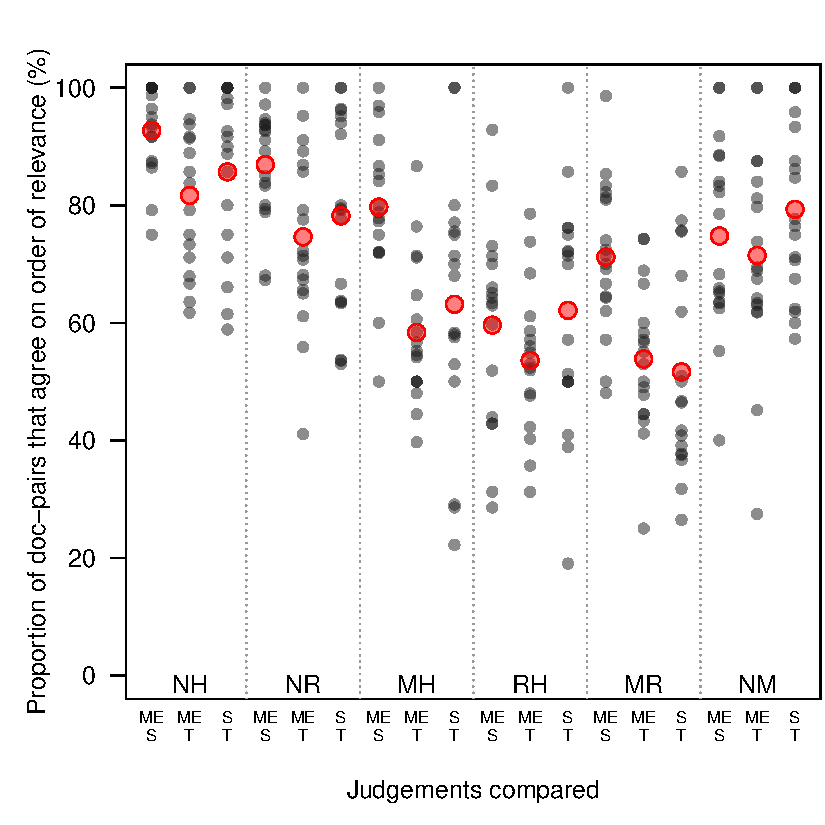
\includegraphics[width=.7\linewidth]{figs/pairwiseSummary2.pdf}
  \vspace{-0.5cm}
  \caption{Agreement on the ordering of relevance of all document pairs (one
small dot per topic) between judges as indicated on the x-axis (ME: magnitude
estimation, S: Sormunen and T: TREC). The large (red) dot is the mean over all topics.
  \label{fig:agreement}}
\end{figure}

It is well-known that relevance is subjective, even when focusing on
``topical'' relevance as is typically done in evaluation campaigns such
as TREC, and that judges will therefore not perfectly agree.
To investigate the level of agreement when using different scales for
judging relevance, we compare the pairwise orderings between binary,
ordinal and magnitude estimation relevance judgments.
Figure~\ref{fig:agreement} shows the proportion of document pairs that
agree on the order of relevance.
For example, when comparing ordinal and magnitude estimation ratings,
if two documents are rated \nn and \mm, and the corresponding magnitude
estimation score of the first is lower than or equal to the score for
the second, this would be an agreement, while if the magnitude
estimation score was higher for the second document, it would indicate
disagreement.
The figure shows the pairwise agreement proportions between magnitude
estimation (ME), Sormunen (S) and TREC (T), for each of the six
possible combinations of ordinal relevance levels.
Red circles indicate the mean score for each group.
It can be seen that the rates of agreement are highly consistent when
comparing any of the three relevance scales.
In particular, ME leads to a higher average agreement with Sormunen than
TREC with Sormunen for documents in the \nn\hh, \nn\rr, \mm\hh, and 
\mm\rr pairs, and slightly lower for \rr\hh and \nn\mm: it can be said
that normalized ME scores agree, in terms of ranks, with Sormunen at
least as well as TREC agrees with Sormunen.
Across all groups, the overall average agreement rates are 77\%
between magnitude estimation and Sormunen, 
64\% between magnitude estimation and TREC, and 65\%
between Sormunen and TREC.
This further supports the validity of the magnitude estimation approach
for gathering relevance judgments.



\subsection{Failure Analysis}
\label{sec:failure-analysis}

Despite the similar overall levels of agreement between the magnitude
estimation method and ordinal relevance,
Figures~\ref{fig:ME-distribution}
and~\ref{fig:ME-distribution-breakdown} show that some individual
documents appear to be ``misjudged''.
We therefore conducted a failure analysis, manually examining a subset
of documents for which the Sormunen relevance level and the median
magnitude estimation scores were substantially different (for example,
where a particular document was assigned an ordinal Sormunen relevance
level of \nn, but the median magnitude estimation score for the
document was closer to the magnitude estimation scores assigned to \hh
documents for the same topic, and substantially higher than the
magnitude estimation scores assigned to other \nn documents for
the same topic).
Based on the manual examination of 34 documents where there appeared to
be a significant flip between the ordinal and magnitude estimation
scores, we found two broad classes of disagreements: those where one
group of assessors appeared to be clearly wrong; and a class
where the topic statement itself is so unclear as to be open to
interpretation.

Of 34 documents that were examined, we found 14 cases (41.2\%) where
the Sormunen ordinal judgments appeared clearly wrong, and 9 (26.5\%)
of cases where the crowd-based magnitude estimation assessments
appeared clearly wrong.
For this class of clear disagreements, where some assessors appear to
be clearly wrong in the assignment of relevance (whether ordinal or
magnitude estimation), the cause mostly appears to be that the
assessors have missed or ignored a specific restriction included as
part of the TREC topic.
For example, the narrative of topic 410, \emph{``Schengen agreement''},
includes the statement that: \emph{``Relevant documents will contain
any information about the actions of signatories of the Schengen
agreement such as: measures to eliminate border controls...''}.
Document {\tt FT932-17156} makes clear reference to nine signatories of
Schengen, and the process of removing passport checks.
As such, it seems implausible that the document should be classed as 
\nn, or completely non-relevant. The original TREC binary judgment
supports this view, having assigned a rating of 1 (indicating that the
document is at least marginally relevant).

For the remaining 11 (32.4\%) of cases, it was not possible to
determine that one assessment was clearly correct and the
other wrong.
Here, the original TREC topic statement itself was ambiguous,
preventing a clear conclusion to be drawn based on the limited
information that the topic statement provided.
For example, a number of topics list several concepts in the narrative
about what is or is not deemed relevant.
However, they introduce ambiguity about whether the document must meet
all of the listed criteria, or whether a subset is sufficient.
For example, topic 407, \emph{``poaching, wildlife preserves''}, states
that 
\emph{``A relevant document must discuss poaching in wildlife
preserves, not in the wild itself.
Also deemed relevant is evidence of preventive measures being taken by
local authorities.''} This raises the ambiguity of whether preventative
measures by authorities against poaching, but not specifically in
wildlife preserves, should be considered as being at least somewhat
relevant,
or completely non-relevant.
We note that further ambiguity is introduced due to the temporal
mismatch between the time when the documents and topics were written (1990s),
and when the magnitude estimation judgments are being made (2010s).
This is particularly the case for topics that include terms such as
``current''.

The above failure analysis must also be interpreted in the context 
that it is known that assessors make mistakes when judging, perhaps
due to fatigue or other lapses in attention, leading to
self-in{\-}con{\-}sistencies~\cite{CarSob10,SchTur11}; or they may display
systematic errors due to a misunderstanding of the relevance criteria, or
relevance drift~\cite{WebPic13}.
Clearly, assessor errors will lower overall agreement rates when
comparing assessments. Determining whether magnitude estimation relevance
assessments lead to higher or lower error rates compared to using
ordinal or binary
 scales is left
for future
work.

Overall, the examination of a set of clear disagreements demonstrates
that there are cases where both groups of assessors (ordinal or
magnitude estimation) are at odds with certain details of the TREC
topic statements, and that these appear to occur at broadly similar
rates. 
Moreover, the topic statements themselves are sometimes a cause of
ambiguity, placing a practical upper-limit on the agreement that can
be achieved.
We conclude therefore that the magnitude estimation relevance
judgments are sound and sensible, having similar agreement rates with
the ordinal Sormunen judgments as the Sormunen judgments have with
TREC assessments. 

\subsection{Judge Variability and Workers Quality [2pg]}
\label{sec:workers-quality}

\sm{move this section before Section~\ref{sec:judge-agreement}, or
  merge with it?}

It is %also 
interesting to study the agreement within the group of the
ten workers judging the same topic/document pair. 
In an attempt to avoid confusion, we speak of \emph{variability} in
this case, and reserve the term ``agreement'' for the agreement of our
judges with the official TREC and Sormunen ones
(Section~\ref{sec:judge-agreement}).
\sm{OR: external agreement, internal agreement, individual agreement?}
In our data, the source of variability might be threefold: (i) the
arbitrary inner scale used by a judge when expressing an ME score;
(ii) the subjective nature of relevance; and (iii) the often feared
low quality of work in crowdsourcing exercises. 
The first has been already discussed and it is removed by the
geometric average normalization process
(Section~\ref{sec:score-normalization}). 
The second is a feature that one might not want to remove from the
data: different judges can truly have different opinions on the
relevance of a document, whatever scale of measurement is used. 
We can nevertheless assume that in our TREC-like scenario it has no
significant effect. 
Of course, the third source is in need of particular attention. 

One way to measure judge reliability is by looking at how different
are the maximum and minimum normalized scores for each topic /
document pair. 
Being on a ratio scale, this can be measured by the ratio
$\max(s'_i) / \min(s'_i)$. 
Figure~\ref{fig:judgeVariability} shows that for most of the 4269
documents this ratio is quite low: for 57\% of the documents it is
$\leq 10$, and for 78\% it is $\leq 20$.
Another measure of dispersion that can be used is the geometric
standard deviation (a version of standard deviation adapted for
geometric mean and log-normal distributions). 
The chart on the right of the figure shows that the geometric standard
deviation correlates quite well with the max/min ratio (Pearson's
correlation is $0.999$), and therefore is an almost equivalent
measure. 
Overall, the data show a not negligible but reasonably low variability.

\begin{figure}[tp]
  \centering
  \includegraphics[width=.9\linewidth,page=6]{figs/JudgeVariability.pdf}
%  \includegraphics[width=.29\linewidth,page=2]{figs/MaxMin-gsd_corr.pdf}
  \caption{Number of documents with a particular
    $\max(s_i) / \min(s_i)$ ratio, out of 4269 documents. 
    In the inner panel, the scatterplot showing the correlation between the
    $\max(s_i) / \min(s_i)$ ratio and geometric standard deviation
    (log scale; 7
    points are left out; the blue dots on the bottom are the 34 out of
    the 36 \nkn and \hkh documents, which received many more judgments
    and therefore exhibit a higher ratio).
    \label{fig:judgeVariability}}
\end{figure}


\begin{figure}[tp]
  \centering
  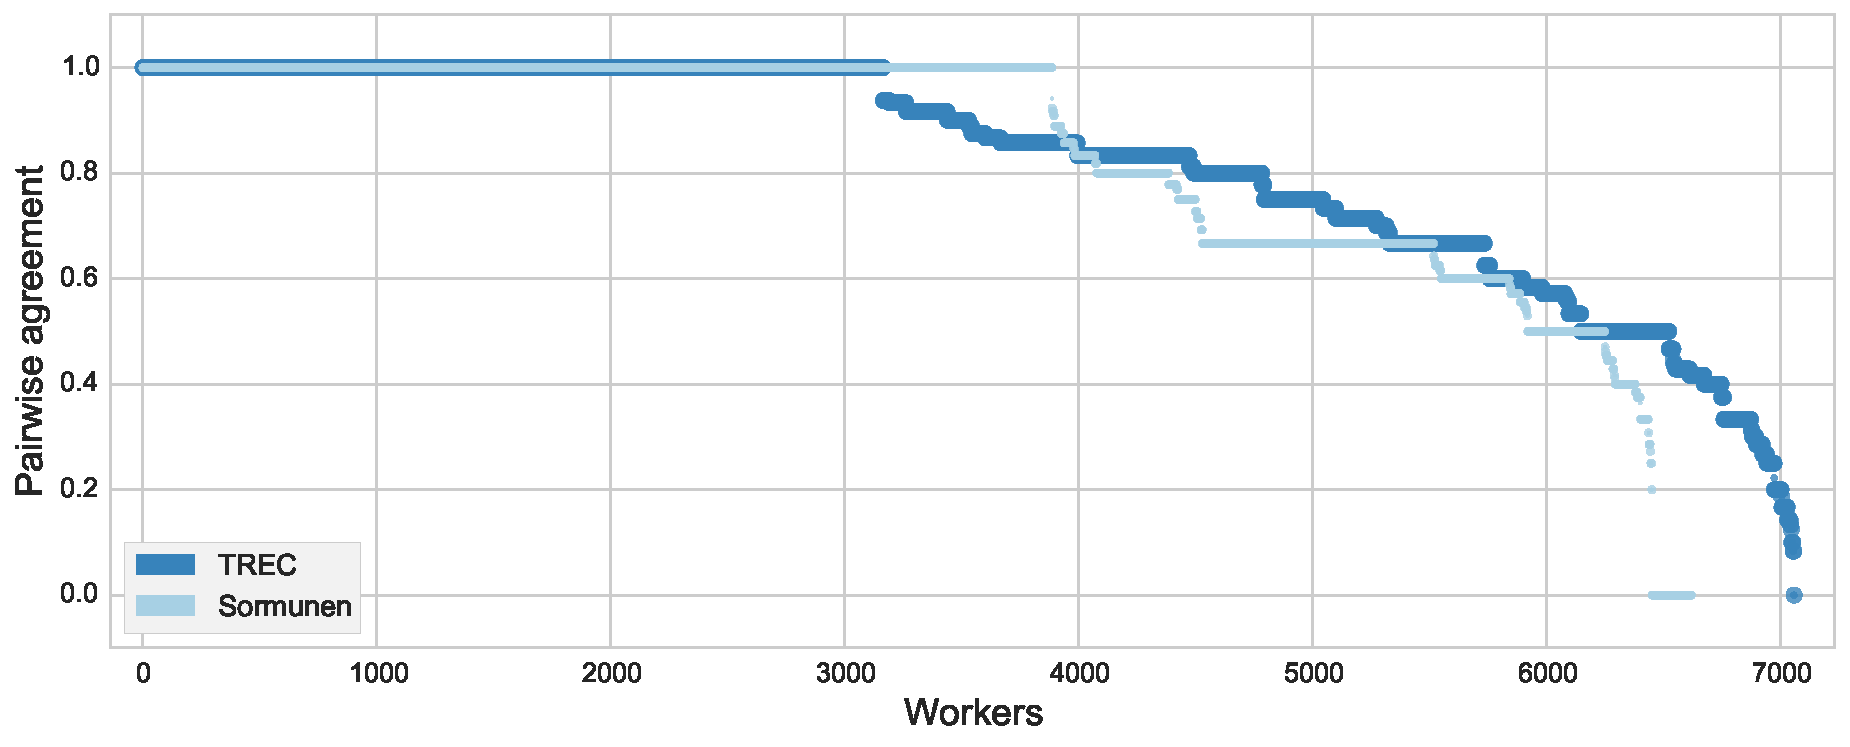
\includegraphics[width=.9\linewidth]{figs/WorkersQuality.png}
  \caption{.
    \label{fig:workersQuality}}
\end{figure}

\begin{itemize}
\item Def.: A worker has a higher quality if the number of pairs of
  docs
  are ordered as in TREC (i.e., fewer swaps)

\item E: For each worker, within a topic, quality is the ratio between
  the correct swaps of documents (according with TREC or Sormunen) and
  all possible swaps for that worker (note: a worker might have fewer
  documents judged by TREC/Sormunen than another one).

\item Workers are generally good. 
\item What happens if we chunk the low quality workers? 
  That would be interesting because we need to disentangle the effect
  of crowdsourcing (low quality, cheating, etc) and the ME effects
  (can the scores be reliable? 
  How? 
  When?)
\end{itemize}

\sm{Maybe better a single section:}
\sm{remember to change judge variability later on}
\subsection{Judge Agreement and Quality [2pg]}

\subsubsection{Internal Agreement}
\label{sec:internal-agreement}

\subsubsection{External Agreement and Workers Quality}
\label{sec:external-agreement}

We now turn to analyze the external agreement, namely the agreement
with the ``official'' TREC and Sormunen judges. We therefore 


\sm{do workers agree among themselves?}

\sm{TODO}
\begin{itemize}
\item Workers quality, variability/agreement/etc.
\item  recommendations on worker quality/number/….
\item What if we use fewer workers?
\item Hmmmm... Distinguish:
  \begin{itemize}
  \item internal variability/agreement (within one worker)
  \item group variability agreement (the group of workers judging the same [t,d] pair)
  \item agreement with expert judges (TREC, Sormunen). Already done.
    Add some more?!
  \item \sm{We briefly go back to normalization and aggregation
      issues. Figure  (add Eddy's chart) shows the effect of different
      normalization and aggregation functions on the quality of the
      workers measured as the number of swaps. As we have discussed in
      Sections~\ref{sec:score-distribution}
      and~\ref{sec:score-normalization}, we decided to use geometric
      averaging and median normalized score...}
    \sm{hmmmm here or in Judge Agreement??}
  \end{itemize}

\end{itemize}

% Local Variables:
% TeX-master: "ME-TOIS.tex"
% End:
